\section{Inserting Vertices}
\label{sect:inserting-vertices}

When a new cluster appears in our underlying data set, we want to add a new vertex to the cluster graph. We distinguish between adding a new vertex on the inside and adding a new vertex on the outside because different rules apply.



\paragraph{Inserting Vertices Inside}

First, let us discuss adding a vertex on the inside. All internal faces of the cluster graph are triangles. If we add a vertex in one of the triangular faces, we must also add edges to the three vertices bounding the face without introducing edge crossings in order to preserve the graph's internal triangulatedness. A valid vertex insertion is illustrated in \cref{}.

\begin{figure}[H]
	\centering
	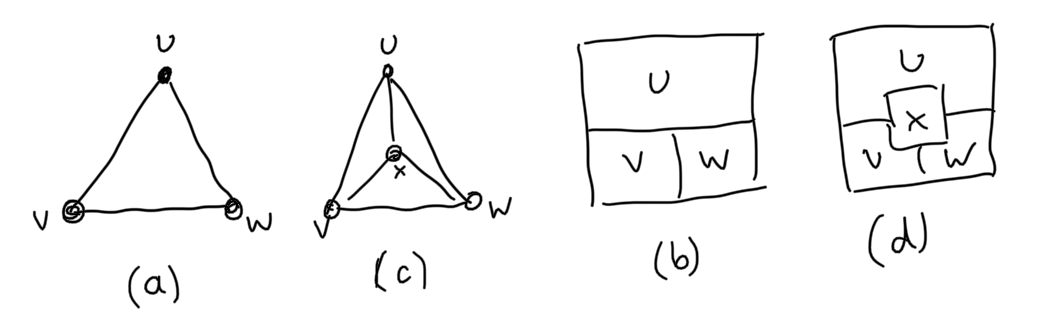
\includegraphics[height=30mm]{Resources/InsertVertexInside.png}
	\caption{A cluster graph and a polygonal dual thereof, before (a, b) and after (c, d) inserting the vertex $x$ in the triangular face $uvw$.}
	\label{fig:insert-vertex-inside-example}
\end{figure}



Let $u$, $v$, and $w$ be the vertices bounding an internal face and $x$ the new vertex we want to add inside said face.

\begin{itemize}
	\item compute three incident boundaries ($u$-$v$, $v$-$w$, $w$-$u$)
	\item on all boundaries, pick the subdivision vertex closest (graph-theoretic) to vertex where all three corresponding faces meet. or create it on midpoint if boundary is only a single edge.
	\item we want to add edges between these subdivision vertices and remove their connections to meeting point instead.
	\item we may need a bend per edge! for each edge, distinguish two cases based on angle at meeting point
	\item if >180, just use meeting as bend loc. otherwise do binary search on segment from meeting point to midpoint of subdivs, starting at far end.
\end{itemize}


\paragraph{Inserting Vertices Outside}

Alternatively, we can add a new vertex in the outer face of the cluster graph. Such a vertex must be connected to at least two vertices on the outer face to preserve the graph's 2-connectivity and its neighbors must form a path on the original boundary of the cluster graph in order not to create holes and thereby violate its internal triangulatedness.

We restrict ourselves to adding new vertices in the outer face that are made incident to exactly 2 neighboring vertices. Let $\{u,v\}$ be an edge on the outer face, then we support adding a new vertex $w$ in the outer face and connecting it to both $u$ and $v$.

\begin{figure}[H]
	\centering
	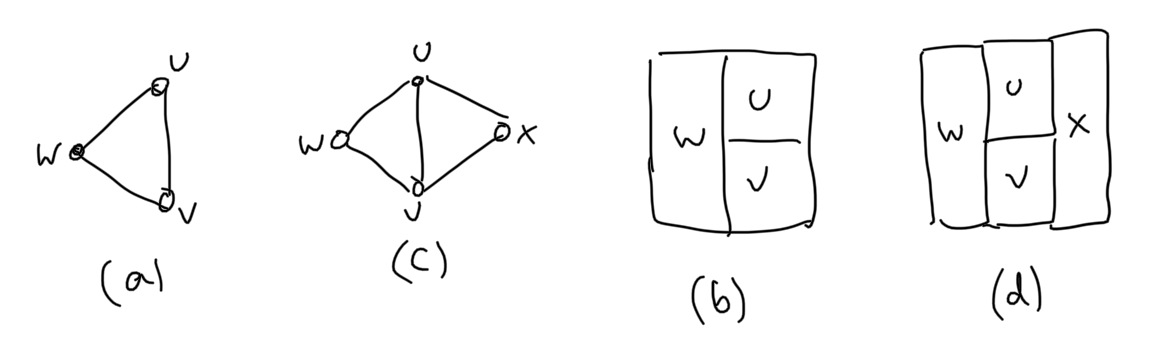
\includegraphics[height=30mm]{Resources/InsertVertexOutside.png}
	\caption{A cluster graph and a polygonal dual thereof, before (a, b) and after (c, d) inserting the vertex $x$ on the outer face and connecting it to $u$ and $v$.}
	\label{fig:insert-vertex-outside-example}
\end{figure}

\begin{itemize}
	\item compute boundaries of $u$ and $v$ with the outer face
	\item on both sides, pick the subdivision vertex closest (graph-theoretic) to the vertex where $u$, $v$, and the outer face meet. or create it on midpoint if a boundary is only single edge.
	\item we want to add edge between those two subdivision vertices. may need to add a bend.
	\item need to distinguish two cases based on external angle at meeting point.
	\item in both cases: binary search for bend location on segment from meeting point to midpoint of segment connecting subdivision vertices.
\end{itemize}
